\chapter{Usage}
\label{chap:Usage}

This chapter demonstrates how different responsive patterns can be achieved using the components provided by the various RespVis modules outlined in Chapter~\ref{chap:Modules}.
The \code{src/examples} directory of the RespVis library contains examples that show how the library can be used to create different kinds of charts with varying degrees of responsive configurations.
Even though users can compose custom charts out of low-level components like Series, Axes, and Legends, all examples in this chapter focus on creating responsive visualizations using high-level Chart Window Components.
These Chart Windows represent convenient interfaces that allow visualization authors to focus on responsive configuration rather than on laborious tasks like setting up a Chart's structure and handling the render processes of their components.

All examples provided by the RespVis library follow the same basic structure outlined in Listing~\ref{list:ExampleStructure}:

\begin{enumerate}

\item 
Import the RespVis CSS file \code{respvis.css}.
This file contains the necessary default styling applied on visualization elements rendered by the RespVis library.

\item
Import D3 and RespVis.
RespVis is a D3 extension library, and therefore the functionality of both libraries needs to be imported from either IIFE or ES modules to create visualizations with RespVis.

\item
Attach a \code{<div>} element to the element into which the Chart Window should be rendered.

\item
Bind a fully-initialized data object to the \code{<div>} element that represents the render configuration of the Chart Window.
This data object is usually created by deriving default properties from a partial object via one of the \code{chartWindowXData} functions.

\item
Render the Chart Window using the appropriate \code{chartWindowXRender} function.

\item
Attach a \code{resize} event listener to the \code{<div>} element.
This event listener should update the Chart Window's bound data object based on media queries and rerender it.
Theoretically, it is possible to use the actual viewport size in pixels for responsive configuration decisions, but it is strongly recommended to use media queries via the \code{window.matchMedia} function instead.
The usage of media queries allows a Chart's JavaScript configuration to be based on the same media queries that might be used for the CSS configuration of the same Chart.


\begin{samepage}
\lstinputlisting[%
  float=tp,
  aboveskip=\floatsep,
  belowskip=\floatsep,
  xleftmargin=0cm,              % no extra margins for floats
  xrightmargin=0cm,             % no extra margins for floats
  %
  basicstyle=\footnotesize\ttfamily,
  frame=shadowbox,
  numbers=left,
  label=list:ExampleStructure,
  caption={[Structure of Examples]%
    The common structure of all responsive examples provided by RespVis.
    Some parts have been removed to not distract from the essential ones.
  },
]{listings/example-structure.html}
\end{samepage}

\end{enumerate}

Since one of the core premises of RespVis is to enable the configuration of SVG-based visualizations with CSS, many responsive patterns can be implemented without JavaScript.
In general, everything that does not affect the content or behavior of a Chart should be handled in CSS, which includes configuring presentation attributes and the layout of laid-out elements.
Configuration changes that affect a Chart's content or behavior, like changing the visualized data, texts, or interaction mechanisms, still need to be applied in JavaScript.
Knowing what kind of configuration is better done in CSS or JavaScript is not immediately obvious and can be confusing to figure out for developers unfamiliar with RespVis.
There are plans to allow configuring even more in CSS, but this requires that data is also accessible there, which would cause a rather extensive refactoring and, therefore, will be considered for a future release of the library.

\section{Axes}
\label{sec:AxesUsage}

Axes are used to visualize the spatial mapping of abstract values by rendering abstract values as ticks at the spatial positions to which they are being mapped.
In addition to ticks, an Axis also contains an optional title and subtitle to describe the visualized data further.
Axis-related responsive patterns are of great significance because nearly every Chart includes Axes, and often improving the responsiveness of Axes alone can already lead to significant improvements in a user's experience.

The following list contains all the responsive patterns that can be applied to Axes and explains how they can be implemented for RespVis visualizations:

\begin{itemize}

\item
Rotate tick labels.
One of the most effective ways to prevent tick labels from overlapping is rotating them by up to 90 degrees because all the available information is preserved and only presented differently.
Tick labels can be rotated by setting a rotation in the CSS \code{transform} property on them and modifying their CSS \code{text-anchor} property accordingly. 

\item
Simplify tick labels.
In some cases rotating tick labels may not be desired, or labels might still overlap after rotation.
The next best thing that can be done in these cases is to shorten tick labels if shorter textual representations exist.
The D3 Axis object used for rendering ticks is accessible via the \code{configureAxis} function property on an Axis' data object, and how individual tick labels are shortened is specified as a formatting callback set via the D3 Axis' \code{tickFormat} function.

\item
Remove ticks.
If neither rotation nor shortening of tick labels is applicable, the last thing that can be done is to reduce the number of ticks shown.
This can be achieved either via a D3 Axis' \code{ticks} or \code{tickValues} function, or via the CSS \code{display} property.
A D3 Axis' \code{ticks} function allows specifying the desired number of ticks that shall be rendered, and the D3 Axis' render function will decide how many ticks to create based on this number and other contributing factors.
The \code{tickValues} function of a D3 Axis allows for much more control than the \code{ticks} function because it is used to specify the exact abstract values for which ticks shall be rendered.

\item
Simplify title/subtitle.
Since Axes do not just contain ticks but also titles and subtitles, these should not be ignored when optimizing the responsiveness of Axes.
One of the things that can be done is to simplify titles/subtitles by specifying shorter textual representations via the \code{title} and \code{subtitle} properties on Axes' data objects.

\item
Relocate title/subtitle.
The titles and subtitles of Axes can be relocated by modifying the Axes' grid layouts via the CSS \code{grid-template} property. 

\item
Remove title/subtitle.
The titles and subtitles of Axes can be hidden via the CSS \code{display} property.

\end{itemize}

\section{Legends}
\label{sec:LegendsUsage}

Legends visualize the non-spatial mapping of abstract values such as mappings to colors, shapes, and sizes via labeled symbols and are needed in any visualization that uses such encodings.
They are essential and frequently encountered parts of visualizations and, as such, must not be ignored when optimizing a visualization's responsiveness. 

The following list shows how different responsive patterns that can be applied to Legends are implemented for RespVis visualizations: 

\begin{itemize}

\item
Relocate Legend.
A Legend's position in its containing Chart can be controlled by directly modifying the Chart's grid layout via the CSS \code{grid-template} property, or by positioning the Legend at predefined \code{\"top\"}, \code{\"right\"}, \code{\"bottom\"}, and \code{\"left\"} positions via the \code{data-legend-position} attribute.

\item
Simplify title.
A Legend's title can be shortened by specifying a shorter textual representation for it via the \code{title} property on a Chart's data object.

\item
Remove title.
If the title can not be further shortened or if it does not convey too much important information, it can be hidden via the CSS \code{display} property.

\item
Simplify symbol labels.
If the symbol labels can be shortened, this can be done via the \code{labels} property on a Legend's data object.
This property allows the specification of the text content of all labels as an array of string values.

\item
Relocate labeled symbols.
Changing the layout of labeled symbols is one of the most effective responsive patterns applicable to Legends.
By default, labeled symbols are laid out using CSS Flexbox layouting.
Thus, whether labeled symbols are laid out horizontally or vertically can be controlled using the CSS \code{flex-direction} property on their container element.

\end{itemize}

\section{Bar Charts}
\label{sec:BarChartsUsage}

Bar Charts are used to compare categories associated with quantitative values by visualizing them as bars whose lengths depend on the quantitative dimension of the data.
In the case of Multi-Series Bar Charts like Grouped and Stacked Bar Charts, categories are further divided into subcategories associated with quantitative values and compared with one another rather than categories themselves.
Bars in Multi-Series Bar Charts are usually colored based on their subcategories which is why these Charts often include Legends to visualize this color encoding.

The different responsive patterns applicable to Bar Charts have already been discussed in Section~\ref{sec:BarChartExamples}, and the focus here lies on demonstrating their implementation using RespVis Bar Chart Windows.
Listing~\ref{list:BarChartPatterns} demonstrates how some of these patterns can be implemented to create the responsive Bar Chart shown in Figure~\ref{fig:BarChartPatterns}.
In practice, the responsive patterns that can be applied to different variants of Bar Charts are very similar, which is why this section does not differentiate between them.

The following list shows the implementation of different responsive patterns that can be applied on RespVis Bar Charts:

\begin{itemize}

\item
Rescale draw area.
Scaling a Bar Chart to fit into the available space is done automatically by their render functions.
By default, Axes and Legends only take up necessary space, and the remaining space is filled with the Chart's draw area.
Bars and labels in this draw area are automatically scaled and positioned to fit into the allocated space.

\item
Reduce bar padding.
Reducing the paddings between bars frees up space that can be used by the bars themselves.
Paddings can be controlled via the \code{padding} function on the \code{categoryScale} property of a Bar Chart's data object. 

\item
Simplify bar labels.
When reducing the width of Bar Charts, bar labels could start overlapping one another, and it might be a good idea to shorten them, if possible. 
These labels can be configured using the \code{labels} property of a Bar Chart's data object.

\item
Remove bar labels.
An alternative to prevent bar labels from overlapping is to hide some or even all of them.
The best way of implementing this is to hide them via the CSS \code{opacity} or \code{display} properties.

\item
Transpose Chart.
By default, Bar Charts are rendered with vertical bars, and transposing would make them horizontal.
Horizontal Bar Charts are better suited for narrow spaces because bar labels and the tick labels of the Axis representing categories are easier to place.
Furthermore, Horizontal Bar Charts are allowed to extend outside the visible viewport because vertical scrolling is strongly preferred over horizontal scrolling.
Bar Charts can be transposed by setting the \code{flipped} property on their data objects.

\item
Remove bars.
Sometimes it might be required to reduce the number of bars to maintain a good user experience.
Bars representing certain categories or subcategories can be hidden by declaring them as inactive via the \code{activeCategories} and \code{activeSubcategories} properties on a Bar Chart's data object.
Using these properties is easier than manually adapting the \code{categories}, \code{values}, \code{categoryScale}, and \code{valueScale} properties on the data object.
Furthermore, categories and subcategories that have been hidden via the \code{activeCategories} and \code{activeSubcategories} properties can also be unhidden by users via a Chart's Toolbar if they are interested in the additional data.  

\item
Apply Axis patterns.
Since Bar Charts usually contain two Axes to visualize the spatial mappings of categories and values, all responsive patterns mentioned in Section~\ref{sec:AxesUsage} should also be applied to Bar Charts.

\item
Apply Legend patterns.
For Multi-Series Bar Charts that contain Legends to visualize the color mapping of bars, the responsive patterns mentioned in Section~\ref{sec:LegendsUsage} should be applied.

\end{itemize}


\begin{samepage}
\lstinputlisting[%
  float=tp,
  aboveskip=\floatsep,
  belowskip=\floatsep,
  xleftmargin=0cm,              % no extra margins for floats
  xrightmargin=0cm,             % no extra margins for floats
  %
  basicstyle=\footnotesize\ttfamily,
  frame=shadowbox,
  numbers=left,
  label=list:BarChartPatterns,
  caption={[Implementation of a Responsive RespVis Bar Chart]%
    The implementation of the responsive Bar Chart shown in Figure~\ref{fig:BarChartPatterns}.
    Depending on the screen's width, Axis tick labels are rotated, bar labels are simplified, and on very narrow screens, the whole Chart is transposed.
    Non-essential parts have been removed for clarity reasons.
  },
]{listings/bar-chart-patterns.html}
\end{samepage}

\begin{figure}[tp]
\newcommand{\respscale}{0.5}
\centering
\subfloat[][60rem]{%
  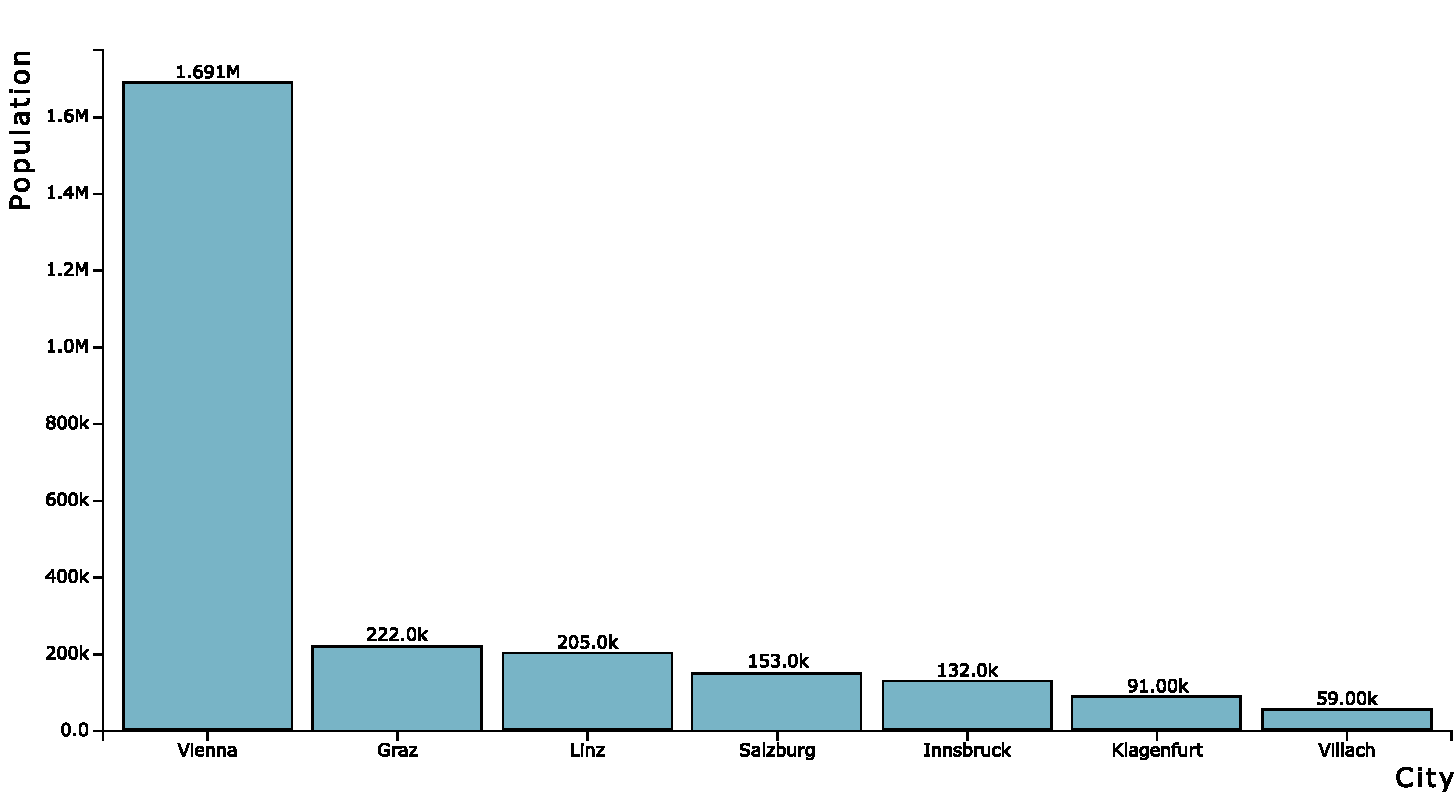
\includegraphics[valign=b,scale=\respscale]{diagrams/respvis-bar-60rem.pdf}%
  \label{fig:BarChartPatterns60rem}%
}
\newline
\subfloat[][40rem]{%
  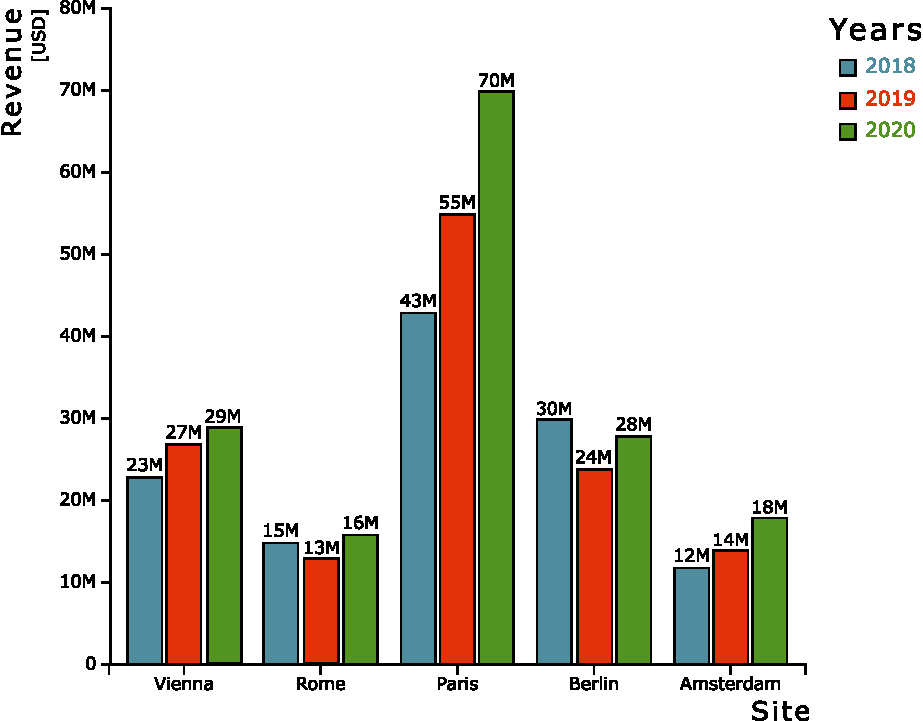
\includegraphics[valign=b,scale=\respscale]{diagrams/respvis-bar-40rem.pdf}%
  \label{fig:BarChartPatterns40rem}%
}
\subfloat[][30rem]{%
  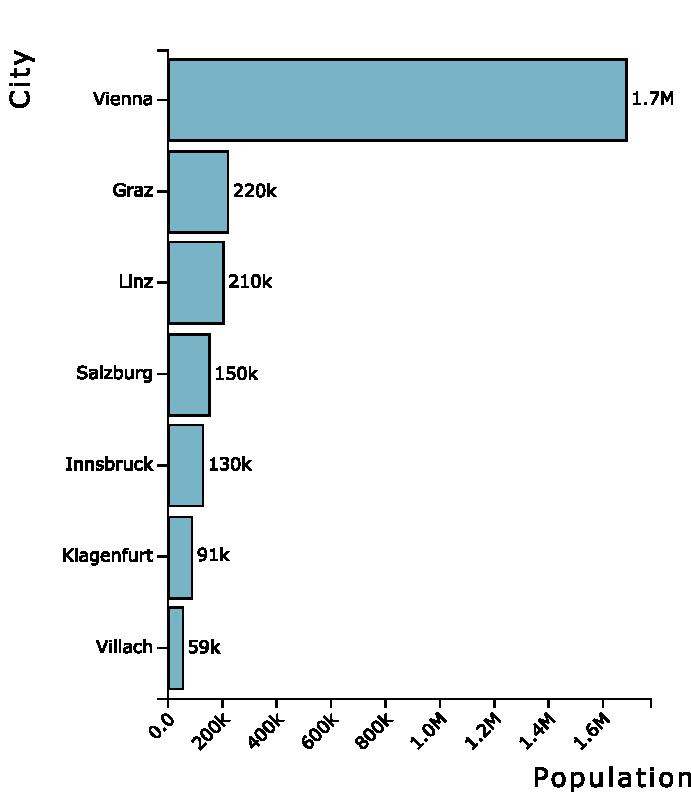
\includegraphics[valign=b,scale=\respscale]{diagrams/respvis-bar-30rem.pdf}%
  \label{fig:BarChartPatterns30rem}%
}
\caption[Responsive RespVis Bar Chart]{
  The resulting responsive Bar Chart that is rendered from the implementation in Listing~\ref{list:BarChartPatterns}.
  \subref{fig:BarChartPatterns60rem} At a viewport size of 60rem, the Chart is not yet transposed, bar labels are shown with a precision of four digits above bars, and tick labels of the bottom axis are not rotated.
  \subref{fig:BarChartPatterns40rem} At a viewport size of 40rem, bar labels are shown with a precision of three digits above bars, and tick labels of the bottom axis are rotated by 45 degrees.
  \subref{fig:BarChartPatterns30rem} At a viewport size of 30rem, the Chart is transposed, bar labels are shown with a precision of two digits to the right of bars, and bottom axis tick labels are still rotated by 45 degrees.
  \imgcredit{Image created by the author of this thesis using RespVis.}
}
\label{fig:BarChartPatterns}
\end{figure}

\section{Line Charts}
\label{sec:LineChartsUsage}

Line Charts are visualizations that show trends in data by plotting markers in regular intervals and connecting them with lines.
It can be distinguished between Single and Multi-Series Line Charts, where Single-Series Line Charts show trends in two-dimensional data via a single line and Multi-Series Line Charts show trends in multi-dimensional data via multiple lines. 
The different lines in Multi-Series Line Charts can be seen as representations of subcategories in the data and are usually colored differently to reflect this.
For this reason, the main difference between Single and Multi-Series Line Charts, apart from rendering multiple lines, is that Multi-Series Line Charts include Legends to visualize the color encoding of subcategories.

The responsive patterns applicable to Line Charts have already been discussed in Section~\ref{sec:LineChartExamples}, and the focus here lies on demonstrating how they can be implemented using RespVis Line Chart Windows. 
For this purpose, Listing~\ref{list:LineChartPatterns} demonstrates how some of these patterns can be combined to create the responsive Line Chart shown in Figure~\ref{fig:LineChartPatterns}.

The following list shows the implementation of different responsive patterns that can be applied on RespVis Line Charts:

\begin{itemize}

\item
Rescale draw area.
As for Bar Charts, Line Charts are automatically scaled by their render functions.
The default behavior is that Axes and potential Legends only take up necessary space, and whatever space is left is filled with the Chart's draw area.
Elements contained in these draw areas like lines, markers, and labels are automatically scaled and positioned to fit into the available space.

\item
Remove markers.
If a Chart contains a large number of individual data points, it might be a good idea to reduce visual clutter by not showing markers for every single one of them.
The best way of removing markers is to hide them via the CSS \code{opacity} or \code{display} properties.

\item
Rescale markers.
An alternative to removing markers is to decrease their sizes.
Marker sizes can be controlled via the \code{markers.radiuses} property on the data objects of Line Charts.

\item
Simplify marker labels.
The labels of markers might start overlapping when trying to fit a Line Chart into increasingly narrow widths.
A good solution for this is to shorten marker labels by providing shorter textual representations for them via the \code{labels} property on a Line Chart's data object.

\item
Remove marker labels.
Sometimes shortening labels may not be possible, desired, or effective enough and an alternative to prevent them from overlapping is to remove some or all of them.
The recommended way to remove marker labels is to hide them via the CSS \code{opacity} or \code{display} properties.

\item
Transpose Chart.
Even though Line Charts are less frequently transposed than Bar Charts, there are still situations when transposing a Line Chart could improve the user's experience.
One such situation would be a Line Chart that includes so many points of data that the density becomes too much for displaying all of it in a Horizontal Line Chart with limited width.
Transposing such a Chart into a Vertical Line Chart could reduce the data density by allowing the Chart to extend outside the visible viewport and having users scroll vertically.
Furthermore, Vertical Line Charts are useful for heavily annotated Line Charts because labels are much easier to place in them than in horizontal ones.
Line Charts can be transposed by setting the \code{flipped} property on their data objects.

\item
Apply Axis patterns.
As with all Charts that use Axes to visualize spatial mappings, the responsive patterns described in Section~\ref{sec:AxesUsage} should be applied to the Axes in Line Charts.
Axes of Line Charts could even be removed completely via the CSS \code{display} property to turn Line Charts into Sparklines, but this should be considered carefully because information about the scale of data is lost when hiding Axes.

\item
Apply Legend patterns.
In Multi-Series Line Charts that contain Legends to visualize non-spatial data encodings, the responsive patterns discussed in Section~\ref{sec:LegendsUsage} should be applied.

\end{itemize}


\begin{samepage}
\lstinputlisting[%
  float=tp,
  aboveskip=\floatsep,
  belowskip=\floatsep,
  xleftmargin=0cm,              % no extra margins for floats
  xrightmargin=0cm,             % no extra margins for floats
  %
  basicstyle=\footnotesize\ttfamily,
  frame=shadowbox,
  numbers=left,
  label=list:LineChartPatterns,
  caption={[Implementation of a Responsive RespVis Line Chart]%
      The implementation of the responsive Line Chart shown in Figure~\ref{fig:LineChartPatterns}. 
      Depending on the screen width, Axis ticks and markers are hidden, Axis tick labels are simplified, and on very narrow screens, Axes are hidden to turn the Line Chart into a Sparkline.
      Non-essential parts of the implementation have been removed for clarity reasons.
  },
]{listings/line-chart-patterns.html}
\end{samepage}

\begin{figure}[tp]
\newcommand{\respscale}{0.5}
\centering
\subfloat[][60rem]{%
  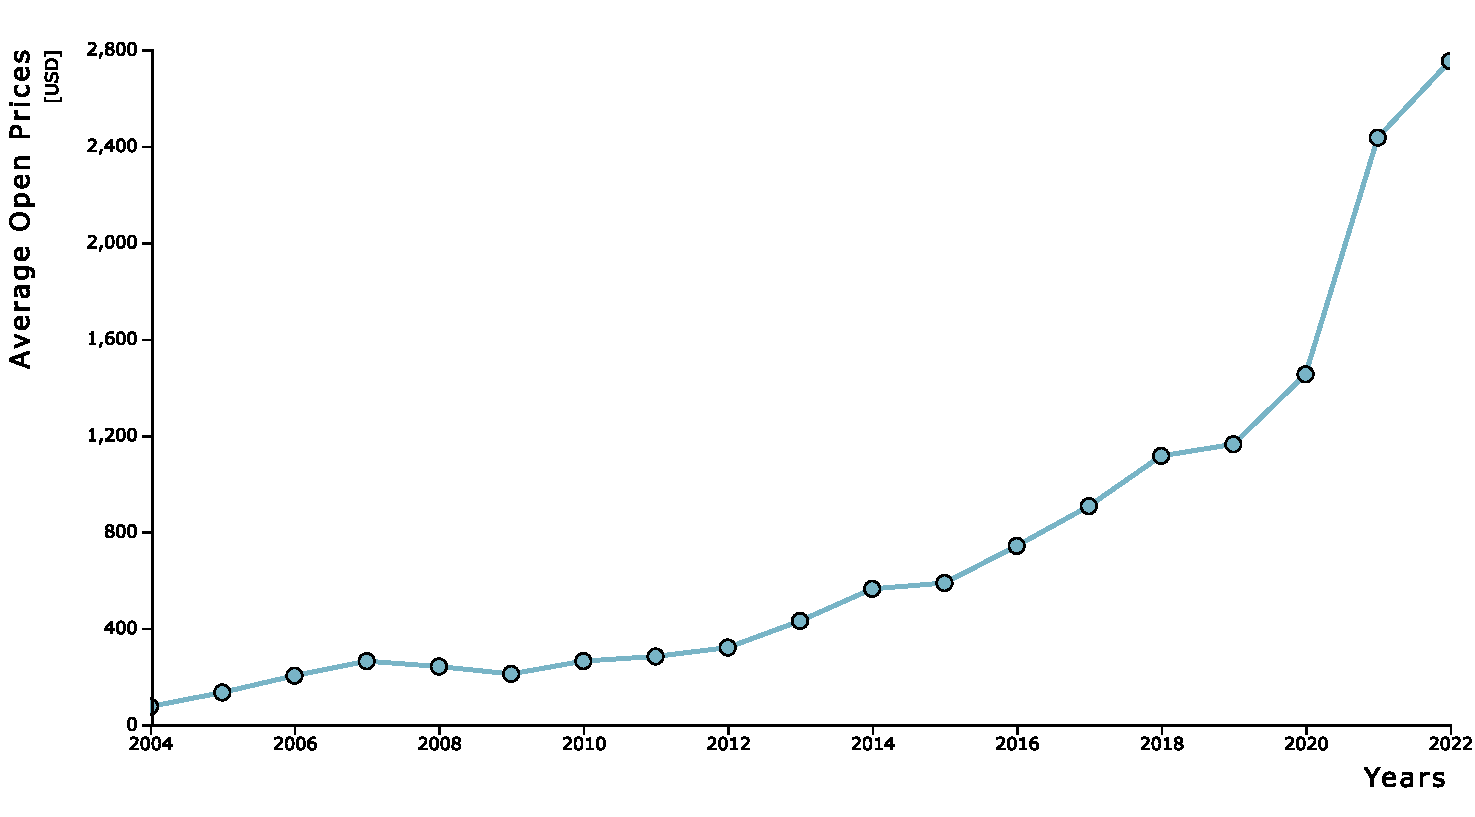
\includegraphics[valign=b,scale=\respscale]{diagrams/respvis-line-60rem.pdf}%
  \label{fig:LineChartPatterns60rem}%
}
\newline
\subfloat[][40rem]{%
  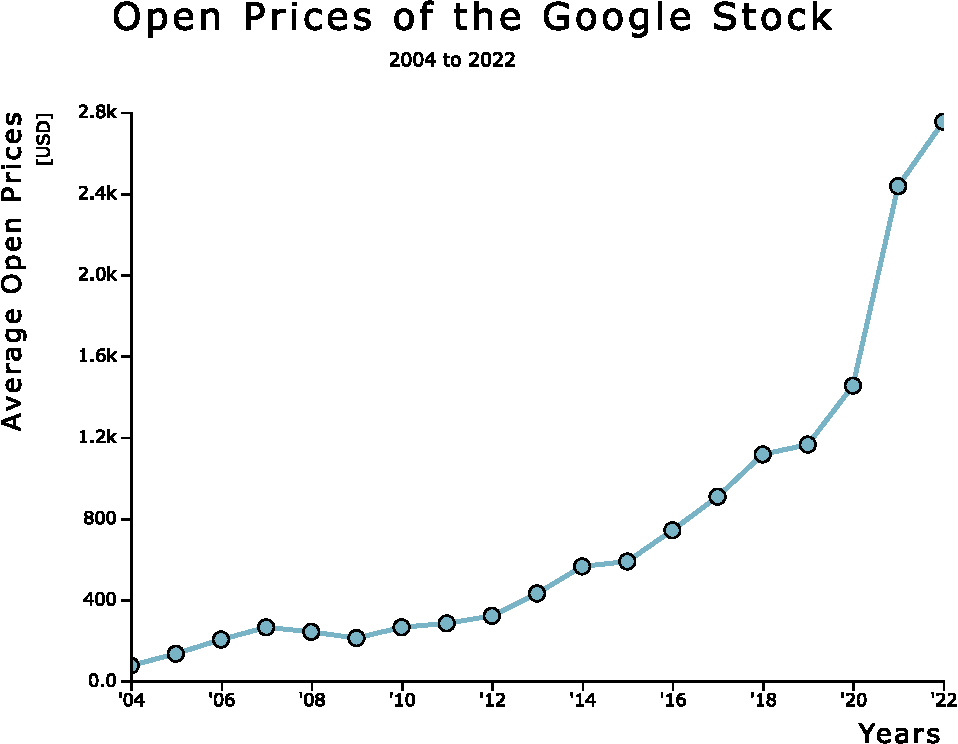
\includegraphics[valign=b,scale=\respscale]{diagrams/respvis-line-40rem.pdf}%
  \label{fig:LineChartPatterns40rem}%
}
\subfloat[][30rem]{%
  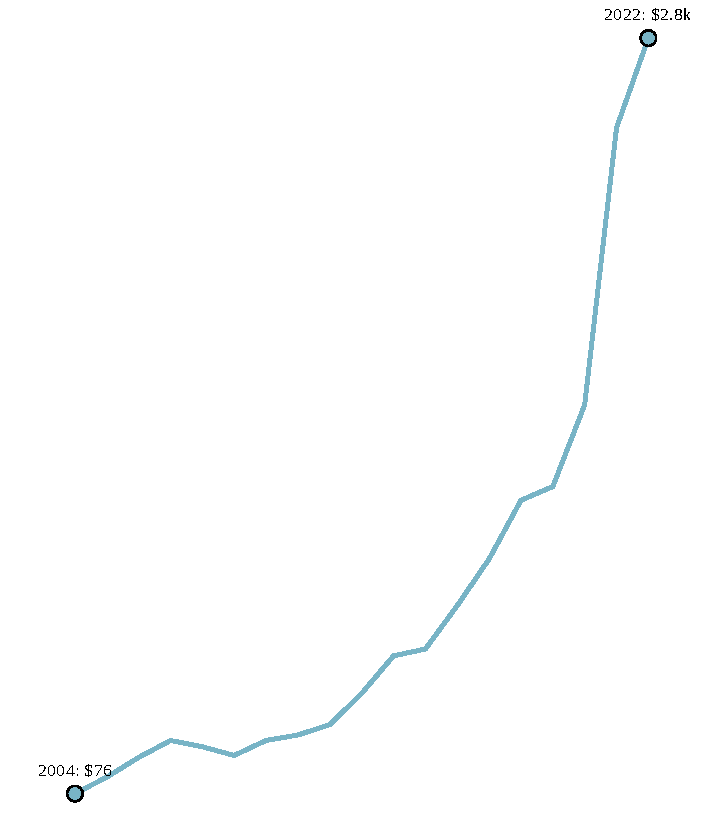
\includegraphics[valign=b,scale=\respscale]{diagrams/respvis-line-30rem.pdf}%
  \label{fig:LineChartPatterns30rem}%
}
\caption[Responsive RespVis Line Chart]{
  The resulting responsive Line Chart that is rendered from the implementation in Listing~\ref{list:LineChartPatterns}.
  \subref{fig:LineChartPatterns60rem} At a viewport size of 60rem, all markers are shown and tick labels are not shortened.
  \subref{fig:LineChartPatterns40rem} At a viewport size of 40rem, tick labels are shortened.
  \subref{fig:LineChartPatterns30rem} At a viewport size of 30rem, Axes are hidden and only the first and last markers and marker labels are shown to turn the Chart into a Sparkline.
  \imgcredit{Image created by the author of this thesis using RespVis.}
}
\label{fig:LineChartPatterns}
\end{figure}

\section{Point Charts}
\label{sec:PointChartsUsage}

Point Charts, sometimes also called Scatterplots, are used to discover patterns and correlations in data by plotting individual data points as points in a Cartesian coordinate system.
In most cases, Point Charts are only used to visualize two-dimensional data by plotting points of the same color, but they can also be used to visualize multi-dimensional data by adding color, size, or shape encodings.
If such additional encodings are used, Point Charts usually include Legends to visualize them. 

The responsive patterns applicable to Point Charts have already been discussed in Section~\ref{sec:ScatterplotExamples}, and the focus here mainly lies on demonstrating their implementation using RespVis Point Chart Windows.
Listing~\ref{list:PointChartPatterns} shows how some of these patterns can be implemented to create the responsive Point Chart displayed in Figure~\ref{fig:PointChartPatterns}.

The following list shows the implementation of different responsive patterns that can be applied on RespVis Point Charts:

\begin{itemize}

\item
Rescale draw area.
As with other Cartesian Charts, the draw areas of Point Charts and their contents are automatically scaled by the Chart's render functions to fill the space not occupied by the Axes and potential Legends of Charts.

\item
Rescale points.
When a large number of points are rendered in a Point Chart, it can be helpful to reduce their sizes to make individual ones easier to see and reduce clutter.
The sizes of points can be controlled via the \code{radiuses} property on the data objects of Point Charts.

\item
Simplify labels.
When labels are shown in a Point Chart, it might be helpful to shorten them when reducing the width of Charts to prevent them from overlapping.
The texts of labels can be configured via the \code{labels} property on the data objects of Point Charts.

\item
Remove labels.
Often, Point Charts are used for the visualization of large data sets.
In such situations, rendering labels for all points would only clutter the visualization, and it might be better to hide them via the CSS \code{opacity} or \code{display} properties. 

\item
Zoom draw area.
Zooming allows users to view data at various levels of detail.
Charts can be zoomed by adjusting the domains of the scales handling the spatial encoding of data, which are the \code{xScale} and \code{yScale} properties on the data objects of Point Charts.
To simplify the setup and handling of the zooming interaction, the D3 Zoom Module \parencite{D3Zoom} can be used, which is demonstrated in detail in Listing~\ref{list:PointChartPatterns}.

\item
Apply Axis patterns.
As with all Cartesian charts that use Axes to visualize spatially-encoded data, the Axis-related responsive patterns described in Section~\ref{sec:AxesUsage} should be applied to Point Charts.

\item
Apply Legend patterns.
In the case of Point Charts that visualize additional non-spatial data encodings with Legends, the responsive patterns discussed in Section~\ref{sec:LegendsUsage} should be applied.  

\end{itemize} 

\begin{samepage}
\lstinputlisting[%
  float=tp,
  aboveskip=\floatsep,
  belowskip=\floatsep,
  xleftmargin=0cm,              % no extra margins for floats
  xrightmargin=0cm,             % no extra margins for floats
  %
  basicstyle=\footnotesize\ttfamily,
  frame=shadowbox,
  numbers=left,
  label=list:PointChartPatterns,
  caption={[Implementation of Responsive RespVis Point Charts]%
    The implementation of the responsive Point Chart shown in Figure~\ref{fig:PointChartPatterns}. 
    Depending on the screen width, Axis ticks are hidden, Axis tick labels are shortened, and point radiuses are reduces.
    Additionally, zooming is implemented using the D3 Zoom package \parencite{D3Zoom}.
    Non-essential parts of the implementation have been removed for clarity reasons.
  },
]{listings/point-chart-patterns.html}
\end{samepage}

\begin{figure}[tp]
\newcommand{\respscale}{0.5}
\centering
\subfloat[][60rem]{%
  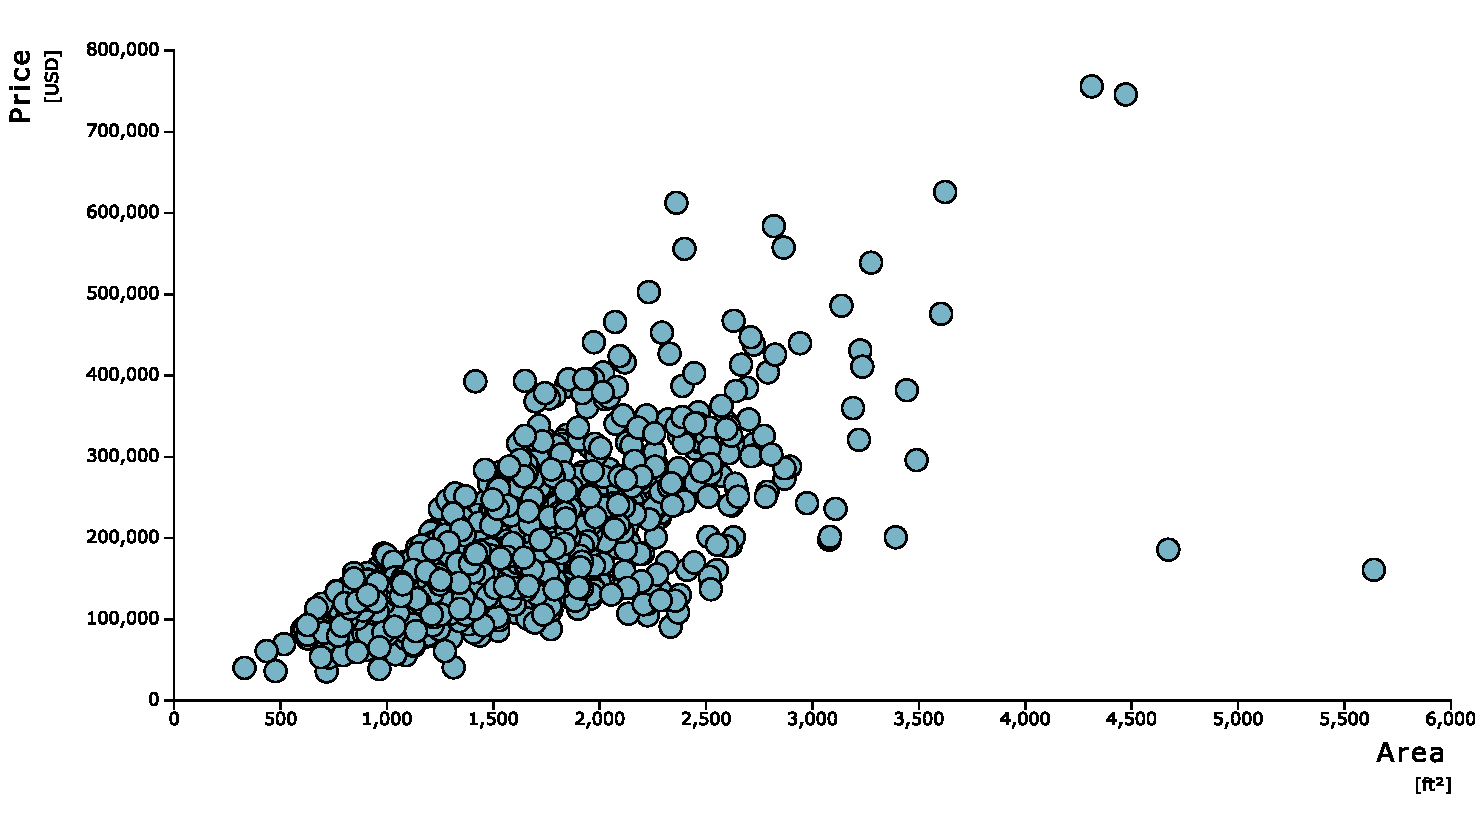
\includegraphics[valign=b,scale=\respscale]{diagrams/respvis-point-60rem.pdf}%
  \label{fig:PointChartPatterns60rem}%
}
\newline
\subfloat[][40rem]{%
  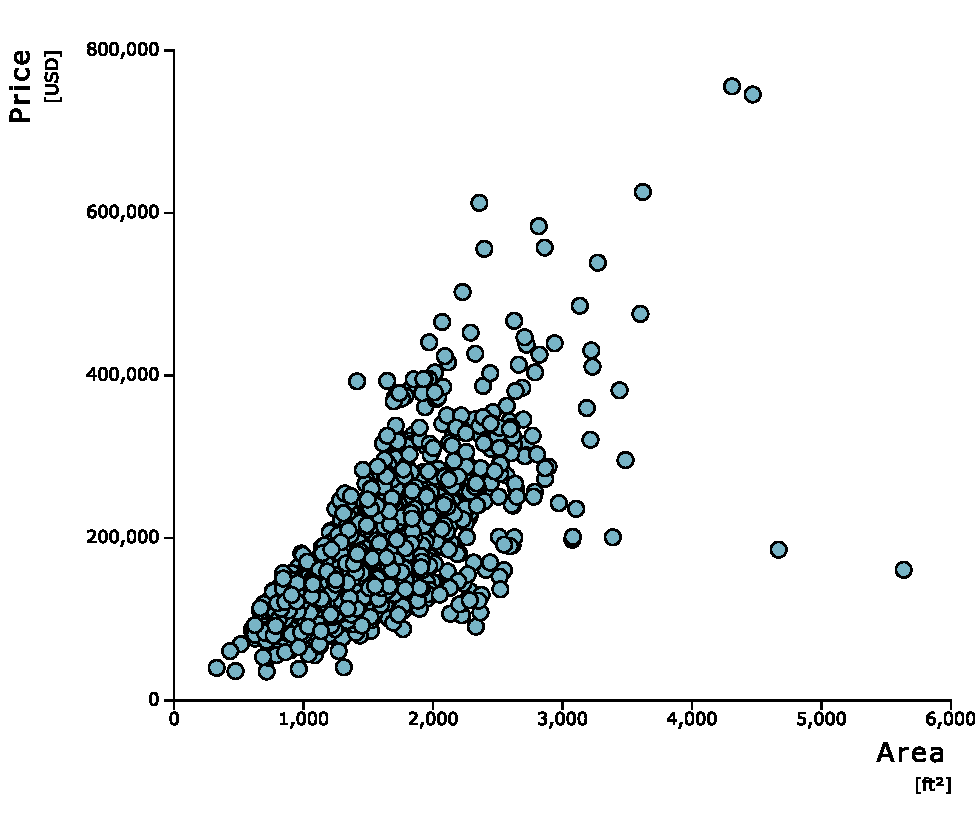
\includegraphics[valign=b,scale=\respscale]{diagrams/respvis-point-40rem.pdf}%
  \label{fig:PointChartPatterns40rem}%
}
% \subfloat[][30rem]{%
%   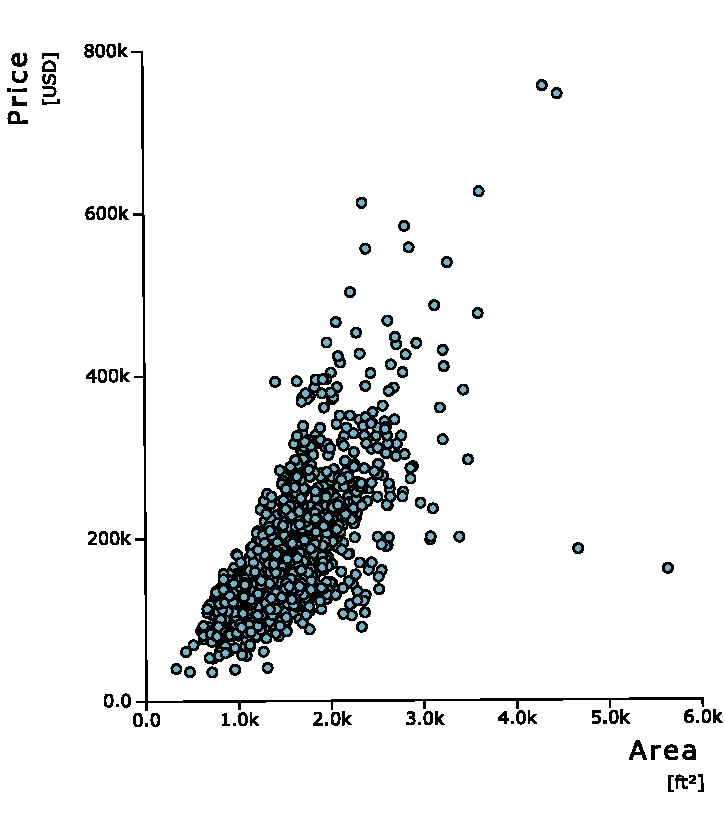
\includegraphics[valign=b,scale=\respscale]{diagrams/respvis-point-30rem.pdf}%
%   \label{fig:PointChartPatterns30rem}%
% }
\subfloat[][30rem, zoomed]{%
  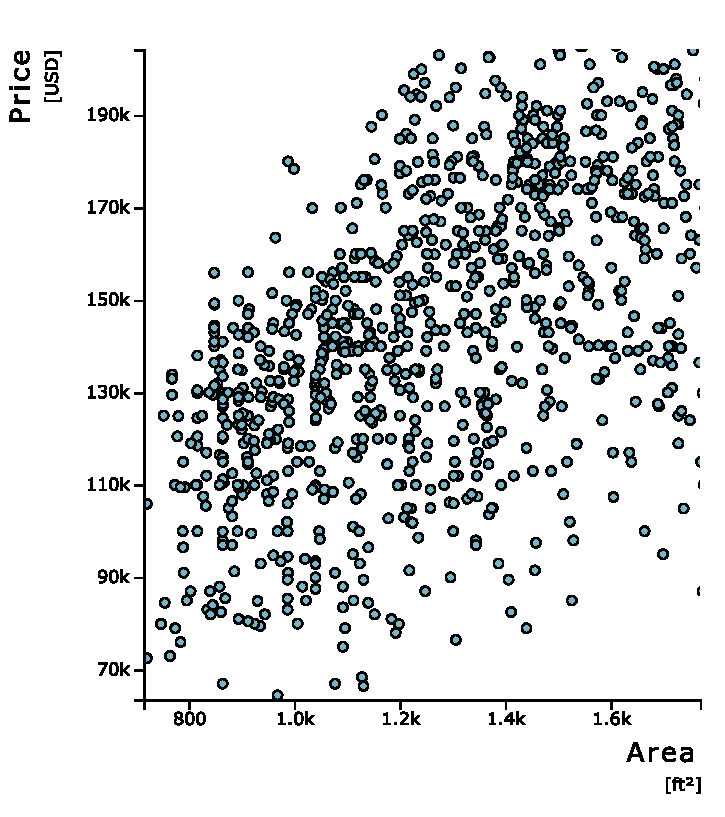
\includegraphics[valign=b,scale=\respscale]{diagrams/respvis-point-30rem-zoomed.pdf}%
  \label{fig:PointChartPatterns30remZoomed}%
}
\caption[Responsive RespVis Point Chart]{
  The resulting responsive Point Chart that is rendered from the implementation in Listing~\ref{list:PointChartPatterns}.
  \subref{fig:PointChartPatterns60rem} At a viewport size of 60rem, all ticks are shown, tick labels are not shortened, and points are rendered at their full size. 
  \subref{fig:PointChartPatterns40rem} At a viewport size of 40rem, only every second tick is shown and point sizes are reduced.
  % \subref{fig:PointChartPatterns30rem} At a viewport size of 30rem,
  \subref{fig:PointChartPatterns30remZoomed} At a viewport size of 30rem, tick labels are shortened using scientific notation and point sizes are further reduced. Additionally, the Chart has been zoomed in.
  \imgcredit{Image created by the author of this thesis using RespVis.}
}
\label{fig:PointChartPatterns}
\end{figure}
